\setcounter{section}{0}

\begin{enumerate}[label=\bfseries Câu \arabic*:]
	\item \mkstar{2}
	
	
	{Hãy chỉ ra điểm đặt, phương, chiều của lực căng trong hình a, b.
		\begin{center}
			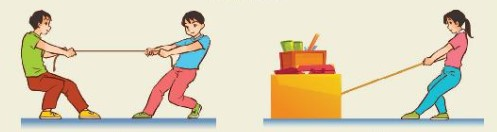
\includegraphics[scale=1]{../figs/VN10-2022-PH-TP019-3.jpg}
		\end{center}
	}
	
	\hideall
	{
		Xác định điểm đặt, phương, chiều của lực căng trong:
		
		- Hình a:
		
		+ Điểm đặt: tại 2 đầu sợi dây.
		
		+ Phương: trùng với phương của sợi dây.
		
		+ Chiều: ngược với chiều của lực do người kéo dãn dây.
		
		- Hình b:
		
		+ Điểm đặt: tại vật.
		
		+ Phương: trùng với phương của sợi dây.
		
		+ Chiều: ngược với chiều của lực do người kéo dãn dây.
	
	}
	\item \mkstar{3}
	
	{
		Lực kế trong hình đang chỉ ở vạch $\SI{10}{N}$.
		\begin{center}
			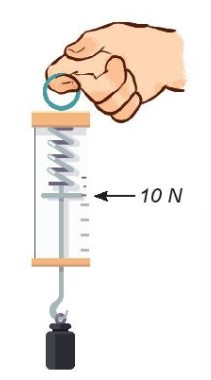
\includegraphics[scale=1]{../figs/VN10-2022-PH-TP019-1.jpg}
		\end{center}
		Tính trọng lượng và khối lược của vật treo và lực kế. Lấy $g \approx \SI{9,8}{m/s}^2$.
			
		
	}
	
	\hideall{
		
		Trọng lượng của vật là $\SI{10}{N}$. Khối lượng của vật là :
			
		$$m= \dfrac{P}{g} = \SI{1,02}{kg}.$$
			
		Vật chịu tác dụng bởi 2 lực cùng phương là lực hút trái đất có chiều từ trên xuống và lức kéo của lò xo có chiều từ dưới lên. 

	}
	
	\item \mkstar{3}
	
	
	{Đo trọng lượng của một vật ở một địa điểm trên Trái Đất có gia tốc rơi tự do là $\SI{9,8}{m/s}^2$, ta được $P = \SI{9,8}{N}$. Nếu đem vật màu tới một địa điểm khác có gia tốc rơi tự do $\SI{9,78}{m/s}^2$ thì khối lượng và trọng lượng của nó đo được là bao nhiêu?
	}
	
	\hideall
	{
		Khối lượng của vật là
		
		$$ m = \dfrac{P}{g} = \SI{1}{kg}.$$
		
		Trọng lượng của vật ở nơi có gia tốc $\SI{9,78}{m/s}^2$ là
		
		$$P= mg = \SI{9,78}{N}.$$
	}
	\item \mkstar{3}
	
	
	{Một bóng đèn có khối lượng $\SI{500}{g}$ được treo thẳng đứng vào trần nhà bằng một sợi dây và đang ở trạng thái cân bằng.
		\begin{enumerate}[label=\alph*)]
			\item Biểu diễn các lực tác dụng lên bóng đèn.
			\item Tính độ lớn của lực căng. 
			\item Nếu dây treo chỉ chịu được một lực căng giới hạn $\SI{5,5}{N}$ thì nó có bị đứt không?
		\end{enumerate}
		
	}
	
	\hideall
	{
		\begin{enumerate}[label=\alph*)]
			\item Các lực tác dụng là: Lực hút của trái đất có chiều từ trên xuống và lực kéo của dây treo có chiều tư dưới lên, và chúng cùng phương.
			
			\item Độ lớn của lực căng dây 
			
			$$P= mg = \SI{4,9}{N}.$$
			
			\item 
			
			Nếu dây treo chỉ chịu được một lực căng giới hạn $\SI{5,5}{N}$, thì nó không bị đứt vì lực kéo của dây vẫn nhỏ hơn lực căng giới hạn.
		\end{enumerate}
	}
	\item \mkstar{3}
	
	
	{Một con khỉ biểu diễn xiếc treo mình cân bằng trên một sợi dây bằng một tay như hình. Hãy cho biết trong hai lực căng xuất hiện trên dây ($\vec T_1$ và $\vec T_2$), lực nào có cường độ lớn hơn? Tại sao?
		\begin{center}
			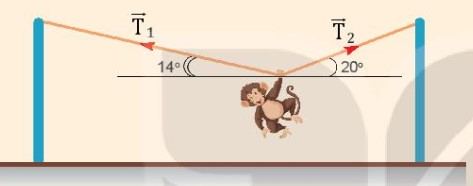
\includegraphics[scale=1]{../figs/VN10-2022-PH-TP019-2.jpg}
		\end{center}
	}
	
	\hideall
	{
		 Lực $\vec T_2$ có độ lớn lớn hơn vì : so với mặt phẳng ngang, góc do lực $T_2$ lớn hơn $T_1$.
	}

	\item \mkstar{4}
	
	
	{
		Vật rắn $\SI{2}{kg}$ nằm cân bằng trên mặt phẳng nghiêng góc $30^\circ$. Lực căng dây có giá trị là bao nhiêu? Lấy $g=\SI{9,8}{m/s}^2$ và bỏ qua ma sát.
		\begin{center}
			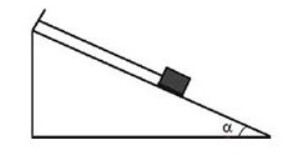
\includegraphics[scale=1]{../figs/VN10-2022-PH-TP019-5.jpg}
		\end{center}
	}
	
	\hideall
	{
		\begin{center}
			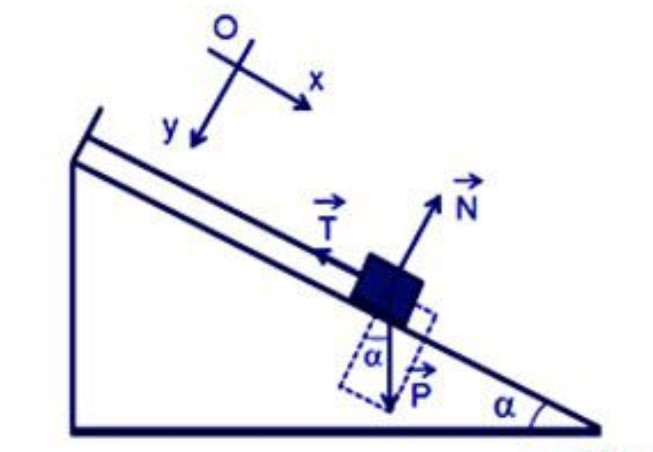
\includegraphics[scale=0.5]{../figs/VN10-2022-PH-TP019-4.jpg}
		\end{center}

	+ Các lực tác dụng lên vật gồm: trọng lực $P$, lực căng dây $T$, phản lực $N$.
	
	+ Ta có:
	
	$$\vec P + \vec T + \vec N = \vec 0\ (1).$$
	
	+ Gắn hệ trục tọa độ, chiếu (1) theo phương Ox, ta được:
	
	$$-T + P_\text{x} = 0 \Rightarrow T = P_\text{x} = P\sin \alpha = mg \sin \alpha = \SI{9,8}{N}.$$
	
	}
	\item \mkstar{4}
	
	
	{
		Một vật rắn khối lượng $\SI{5}{kg}$ được treo cân bằng trên mặt phẳng thẳng đứng bằng một sợi dây như hình vẽ. Bỏ qua ma sát, lấy $g=\SI{9,8}{m/s}^2$; $\alpha = 20^\circ$. Vậy lực căng dây là bao nhiêu?
		\begin{center}
			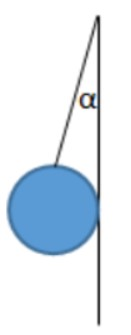
\includegraphics[scale=0.8]{../figs/VN10-2022-PH-TP019-6.jpg}
		\end{center}
	}
	
	\hideall
	{
		\begin{center}
			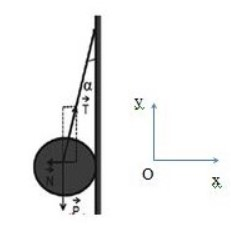
\includegraphics[scale=0.8]{../figs/VN10-2022-PH-TP019-7.jpg}
		\end{center}
		Các lực tác dụng lên vật gồm: trọng lực $P$, lực căng dây $T$ và phản lực $R$ của mặt phẳng thẳng đứng.
		
		Ta có:
		
		$$\vec P + \vec T + \vec N = \vec 0\ (1).$$
		
		Chọn hệ trục Oxy như hình, chiếu (1) theo các phương, ta được:
		
		$$ - P + T\cos \alpha = 0 \Rightarrow T = \dfrac{P}{\cos \alpha} = \SI{52,14}{N}.$$
	}
	\item \mkstar{4}
	
	
	{
		 Treo một vật nặng khối lượng $\SI{6}{kg}$ vào điểm giữa của một sợi dây cáp căng ngang giữa hai cột thẳng đứng cách nhau $\SI{8}{m}$ làm dây võng xuống $\SI{0,5}{m}$. Lấy $g=\SI{10}{m/s}^2$. Tính lực căng của dây.
	}
	
	\hideall
	{
		\begin{center}
			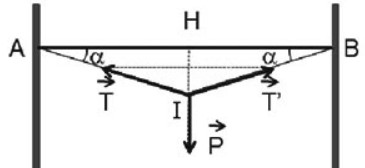
\includegraphics[scale=0.8]{../figs/VN10-2022-PH-TP019-10.jpg}
		\end{center}
	
		Theo đề bài ta có:
		
		$$T = T'; \text{IH} = \SI{0,5}{m}; \text{HA} = \SI{4}{m}.$$
		
		Vật cân bằng:
		
		$$\vec P + \vec T + \vec T' = \vec 0.$$
		
		Từ hình ta có:
		
		$$P = 2T \sin \alpha.$$
		
		Mặt khác, ta có:
		
		$$\tan \alpha = \dfrac{\text{IH}}{\text{HA}} = \dfrac{1}{8} \Rightarrow \sin \alpha = \text{0,124} \Rightarrow T = \dfrac{P}{2\sin \alpha} = \SI{241,9}{N}.$$
	}
		\item \mkstar{4}
	
	
	{
		Vật rắn nằm cân băng như hình vẽ, góc hợp bởi lực căng của dây là $150^\circ$. Tính trọng lượng của vật biết độ lớn lực căng của hai dây là $\SI{200}{N}$.
		\begin{center}
			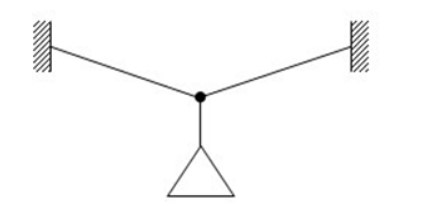
\includegraphics[scale=0.8]{../figs/VN10-2022-PH-TP019-8.jpg}
		\end{center}
	}
	
	\hideall
	{
		\begin{center}
			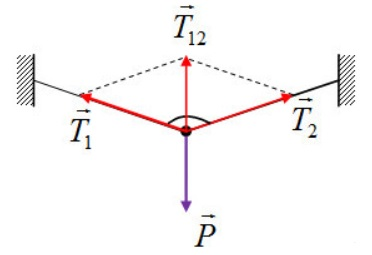
\includegraphics[scale=0.8]{../figs/VN10-2022-PH-TP019-9.jpg}
		\end{center}
	
		Ta có: 
		
		$$T_1 = T_2 = T = \SI{200}{N}.$$
		
		Vật nằm cân bằng nên:
		
		$$\vec T_1 + \vec T_2 + \vec P = \vec 0.$$
		
		Suy ra: 
		
		$$P = T_{12} = 2T \cos \dfrac{\alpha}{2} \approx \SI{103,5}{N}.$$
		
		
	}

		\item \mkstar{4}
	
	{ Một vật có trọng lượng 60N được treo vào vòng nhẫn nhẹ O (coi là chất điểm). Vòng nhẫn được giữ bằng hai dây nhẹ OA và OB. Biết OA nằm ngang còn OB hợp với phương thẳng đứng góc $45^\circ$ (hình vẽ). Tìm lực căng của dây OA và OB.
		\begin{center}
			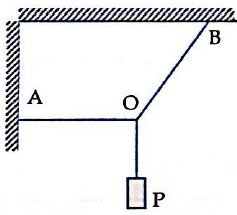
\includegraphics[scale=0.8]{../figs/VN10-2021-PH-TP011-1.jpg}
		\end{center}
	}
	\hideall{
		
		\begin{center}
			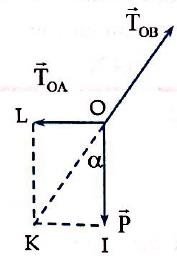
\includegraphics[scale=0.8]{../figs/VN10-2021-PH-TP011-2.jpg}
		\end{center}
		
		Các lực tác dụng vào điểm treo O như hình vẽ.
		
		Góc $\alpha$ là góc giữa OP và OB, $\alpha=45^\circ$.
		$$\text{OI}=\text{OK}\cdot \cos \alpha\Rightarrow \text{OK}=\dfrac{\text{OI}}{\cos \alpha}\Rightarrow T_\text{OB}=\dfrac{P}{\cos \alpha}=60\sqrt{2}\ \text{N} $$.
		
		Tương tự:   $$T_\text{OA}=T_\text{OB}\cdot \sin 45^\circ=60\ \text{N}$$
	}
\end{enumerate}